\documentclass[xcolor=table]{beamer}

% \usepackage{beamerthemesplit} // Activate for custom appearance
%% \usetheme{CambridgeUS}%+
%% \usetheme{Goettingen}%+
%% \usetheme{Marburg}%+
\usepackage[ddmmyyyy]{datetime}
\usepackage[utf8]{inputenc}
\usepackage[T1]{fontenc}
\usepackage[table]{xcolor}
\usepackage{fixltx2e}
\usepackage{float}
\usepackage{wrapfig}
\usepackage{soul}
\usepackage{textcomp}
\usepackage{marvosym}
\usepackage{wasysym}
\usepackage{latexsym}
\usepackage{amssymb}
\usepackage{hyperref}
\usepackage{graphicx}
\usepackage{media9}
\usepackage{minted}

\title{The Julia Language}
\logo{
\includegraphics[width=0.1\textwidth]{logo}}
\author{Dennis Wilson}
\date{\today}

\usepackage{booktabs}
%% \usepackage[natbib=true, bibstyle=authoryear, citestyle=authoryear-comp]{biblatex}
\usepackage{beamerthemesplit}
\newcommand{\Lagr}{\mathcal{L}}
\usetheme{Amsterdam}

\begin{document}

\maketitle
%% \frame{\titlepage}

\frame{\tableofcontents}

\section{Motivation}
\begin{frame}
	\frametitle{Why I use Julia}
  \begin{itemize}
    \item Fast
    \item Plays nice with shell, C/++ and Python
    \item Vectors or loops
    \item Read/Evaluate/Print/Loop (REPL)
    \item Growing ecosystem
  \end{itemize}
\end{frame}

\begin{frame}
	\frametitle{Speed}
  \begin{figure}[ht]
    \centering
    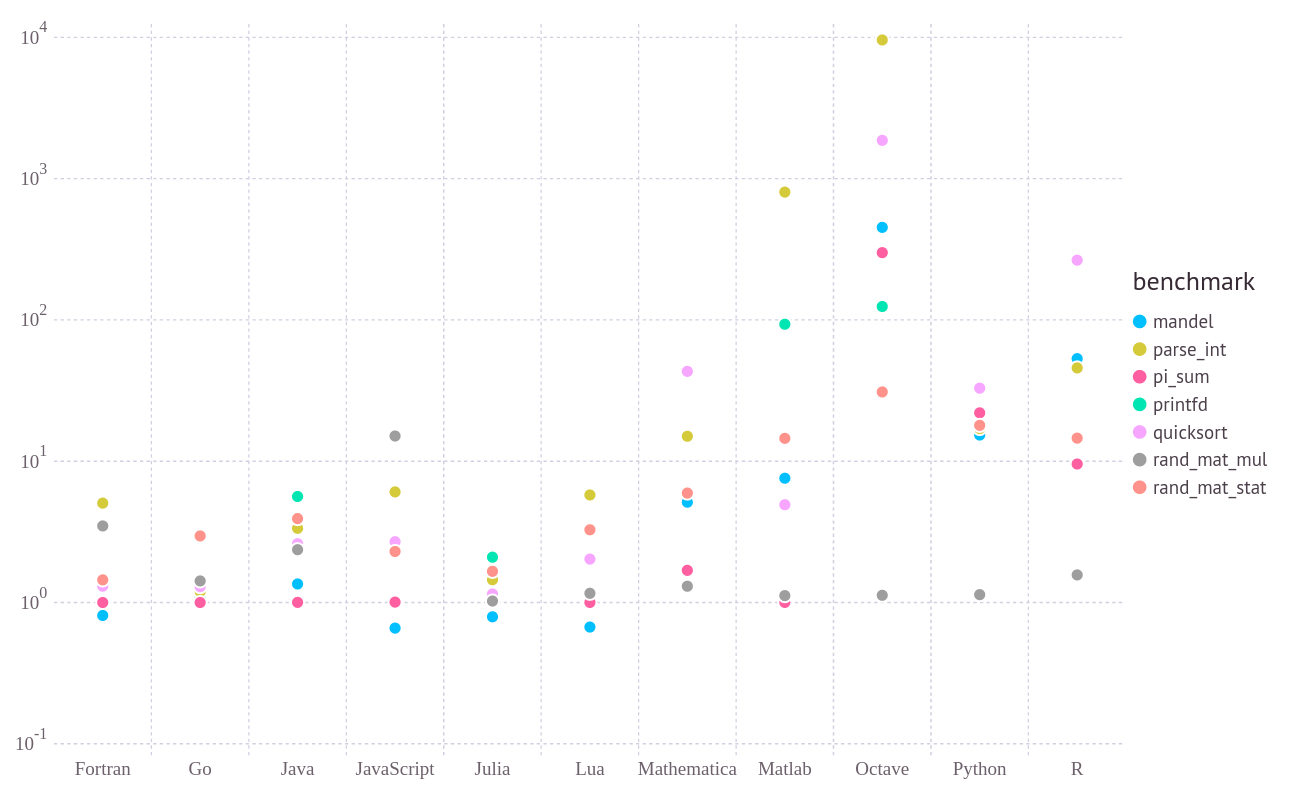
\includegraphics[width=0.8\textwidth]{benchmark}
  \end{figure}
  julialang.org
\end{frame}

\begin{frame}
	\frametitle{Calling C}
  \begin{itemize}
    \begin{small}
    \item \mint{julia}|ccall((symbol, library) or function_pointer, ReturnType,|
      \mint{julia}|(ArgumentType1, ...), ArgumentValue1, ...)|
    \item \mint{julia}|cfunction(function::Function, ReturnType::Type,|
      \mint{julia}|(ArgumentTypes...))|
    \item https://github.com/timholy/Cpp.jl
    \item https://github.com/Keno/Cxx.jl
    \end{small}
  \end{itemize}
\end{frame}

\begin{frame}[fragile]
	\frametitle{Calling C}
  \begin{tiny}
  \begin{minted}{julia}
[d9w@noise julia]$ export FOO=BAR
[d9w@noise julia]$ julia

julia> function getenv(var::AbstractString)
         val = ccall((:getenv, "libc"),
                     Cstring, (Cstring,), var)
         if val == C_NULL
           error("getenv: undefined variable: ", var)
         end
         unsafe_string(val)
       end
getenv (generic function with 1 method)

julia> getenv("FOO")
"BAR"
  \end{minted}
  \end{tiny}
\end{frame}

\begin{frame}[fragile]
	\frametitle{Cpp.jl}
  \begin{tiny}
  \begin{minted}{c}
 int timestwo(int x) {
   return 2*x;
 }

 double timestwo(double x) {
   return 2*x;
 }
  \end{minted}
  \begin{minted}{julia}
julia> x = 3.5
julia> x2 = @cpp ccall((:timestwo, libdemo), Float64, (Float64,), x)
julia> y = 3
julia> y2 = @cpp ccall((:timestwo, libdemo), Int, (Int,), y)
  \end{minted}
  \end{tiny}
\end{frame}

\begin{frame}[fragile]
	\frametitle{Cxx.jl}
  \begin{tiny}
  \begin{minted}{julia}
julia> using Cxx
julia> cxx"""#include <iostream>
       class Hello
       { 
           public:
               void hello_world(const char *now){
                   std::string snow = now;
                   std::cout << "Hello World! Now is " << snow << std::endl;
               }
        };"""
julia> hello_class = @cxxnew Hello()
julia> tstamp = string(Dates.now())
julia> @cxx hello_class -> hello_world(pointer(tstamp))
Hello World! Now is 2015-06-19T11:20:31
  \end{minted}
  \end{tiny}
\end{frame}

\begin{frame}[fragile]
	\frametitle{Calling Julia in C}
  \begin{tiny}
  \begin{minted}{c}
#include <julia.h>

int main(int argc, char *argv[])
{
    /* required: setup the Julia context */
    jl_init(NULL);

    /* run Julia commands */
    jl_eval_string("print(sqrt(2.0))");

    /* strongly recommended: notify Julia that the
         program is about to terminate. this allows
         Julia time to cleanup pending write requests
         and run all finalizers
    */
    jl_atexit_hook(0);
    return 0;
}
  \end{minted}
  \end{tiny}
\end{frame}

\begin{frame}[fragile]
	\frametitle{Calling Python}
  \begin{tiny}
  \begin{minted}{julia}
@pyimport numpy.polynomial as P
@pydef type Doubler <: P.Polynomial
    __init__(self, x=10) = (self[:x] = x)
    my_method(self, arg1::Number) = arg1 + 20
    x2.get(self) = self[:x] * 2
    x2.set!(self, new_val) = (self[:x] = new_val / 2)
end
Doubler()[:x2]
  \end{minted}
  \vspace{2.0mm}
  \begin{minted}{python}
import numpy.polynomial
class Doubler(numpy.polynomial.Polynomial):
    def __init__(self, x=10):
        self.x = x
    def my_method(self, arg1): return arg1 + 20
    @property
    def x2(self): return self.x * 2
    @x2.setter
    def x2(self, new_val):
        self.x = new_val / 2
Doubler().x2
  \end{minted}
  \end{tiny}
  \vspace{5.0mm}
  https://github.com/JuliaPy/PyCall.jl
\end{frame}

\begin{frame}[fragile]
	\frametitle{Vectors and loops}
  \begin{tiny}
  \begin{minted}{julia}
function vectorized()
    a = [1.0, 1.0]
    b = [2.0, 2.0]
    x = [NaN, NaN]

    for i in 1:1000000
        x = a + b
    end

    return
end

function devectorized()
    a = [1.0, 1.0]
    b = [2.0, 2.0]
    x = [NaN, NaN]

    for i in 1:1000000
        for index in 1:2
            x[index] = a[index] + b[index]
        end
    end

    return
end
\end{minted}
\end{tiny}
\end{frame}

\begin{frame}[fragile]
	\frametitle{Vectors and loops}
\begin{table}
\small
\begin{tabular}{*{3}{l}}
Approach & Language & Average Time \\
\hline
Vectorized & R & 0.49 \\
Devectorized & R & 4.72 \\
Vectorized & Julia & 0.24 \\
Devectorized & Julia & 0.0035 \\
\end{tabular}
\end{table}
\end{frame}

\begin{frame}[fragile]
	\frametitle{Vectors and loops}
  \begin{tiny}
  \begin{minted}{julia}
julia> X .= f.(2 .* X.^2 .+ 6 .* X.^3 .- sqrt.(X))

julia> for i in eachindex(X)
    x = X[i]
    X[i] = f(2x^2 + 6x^3 - sqrt(x))
end

julia> [1 2 3] .+ [10,20,30]
3×3 Array{Int64,2}:
 11  12  13
 21  22  23
 31  32  33

julia> s = ["The QUICK Brown", "fox     jumped", "over the LAZY dog."];

julia> s .= replace.(lowercase.(s), r"\s+", "-")
3-element Array{String,1}:
 "the-quick-brown"   
 "fox-jumped"        
 "over-the-lazy-dog."
  \end{minted}
  \end{tiny}
\end{frame}

\section{Tutorial}
\begin{frame}
	\frametitle{A brief Julia tutorial}
  \begin{itemize}
    \item A small taste of Julia's cool features
    \item Personal introduction to Julia assuming background in programming
    \item Many other resources online
    \item http://docs.julialang.org/
    \item https://learnxinyminutes.com/docs/julia/
    \item https://github.com/chrisvoncsefalvay/learn-julia-the-hard-way
    \item https://juliabyexample.helpmanual.io/
  \end{itemize}
\end{frame}

\begin{frame}[fragile]
	\frametitle{Types}
  \begin{tiny}
  \begin{minted}{julia}
julia> type Foo
           bar
           baz::Int
           qux::Float64
       end

julia> foo = Foo("Hello, world.", 23, 1.5)
Foo("Hello, world.",23,1.5)

julia> typeof(foo)
Foo

julia> Foo((), 23.5, 1)
ERROR: InexactError()
 in Foo(::Tuple{}, ::Float64, ::Int64) at ./none:2
 ...

julia> foo.qux = 2
2

julia> foo.bar = 1//2
1//2

julia> typeof(foo.bar)
Rational{Int64}
  \end{minted}
  \end{tiny}
\end{frame}

\begin{frame}[fragile]
	\frametitle{Functions}
  \begin{tiny}
  \begin{minted}{julia}
julia> function add(x, y)
    println("x is $x and y is $y")
    x + y
end

julia> add(5, 6)
"x is 5 and y is 6"
11

# Compact assignment of functions
julia> f_add(x, y) = x + y

julia> f_add(3, 4)
7

julia> f_tuple(x, y) = x + y, x - y

julia> f_tuple(3, 4)
(7, -1)

julia> p1(a...) = +(1,a...)
p1 (generic function with 1 method)

julia> p1(1,2,3)
7
\end{minted}
\end{tiny}
\end{frame}

\begin{frame}[fragile]
	\frametitle{Multiple Dispatch}
  \begin{tiny}
  \begin{minted}{julia}
julia> f(x::Float64, y::Float64) = 2x + y;

julia> f(2.0, 3.0)
7.0

julia> f(2.0, 3)
ERROR: MethodError: no method matching f(::Float64, ::Int64)
Closest candidates are:
  f(::Float64, !Matched::Float64) at none:1
...

julia> f(x::Number, y::Number) = 2x - y;

julia> f(2.0, 3)
1.0

julia> methods(f)
# 2 methods for generic function "f":
f(x::Float64, y::Float64) at none:1
f(x::Number, y::Number) at none:1
  \end{minted}
  \end{tiny}
\end{frame}


\begin{frame}[fragile]
	\frametitle{Multiple Dispatch}
  \begin{tiny}
  \begin{minted}{julia}
 julia> methods(+)
 # 166 methods for generic function "+":
 +(a::Float16, b::Float16) at float16.jl:136
 +(x::Float32, y::Float32) at float.jl:206
 +(x::Float64, y::Float64) at float.jl:207
 +(x::Bool, z::Complex{Bool}) at complex.jl:126
 +(x::Bool, y::Bool) at bool.jl:48
 +(x::Bool) at bool.jl:45
 +{T<:AbstractFloat}(x::Bool, y::T) at bool.jl:55
 +(x::Bool, z::Complex) at complex.jl:133
 +(x::Bool, A::AbstractArray{Bool,N<:Any}) at arraymath.jl:105
 +(x::Char, y::Integer) at char.jl:40
 +{T<:Union{Int128,Int16,Int32,Int64,Int8,UInt128,UInt16,UInt32,UInt64,UInt8}}(x::T, y::T) at int.jl:32
 +(z::Complex, w::Complex) at complex.jl:115
 +(z::Complex, x::Bool) at complex.jl:134
 +(x::Real, z::Complex{Bool}) at complex.jl:140
 +(x::Real, z::Complex) at complex.jl:152
 +(z::Complex, x::Real) at complex.jl:153
 +(x::Rational, y::Rational) at rational.jl:179
 ...
 +(a, b, c, xs...) at operators.jl:119
  \end{minted}
  \end{tiny}
\end{frame}

\begin{frame}[fragile]
	\frametitle{Functions are a type}
  \begin{tiny}
  \begin{minted}{julia}
help?> map
  search: map map! mapfoldr mapfoldl mapslices mapreduce mapreducedim
  pmap Mmap lazymap TypeMapLevel TypeMapEntry

  map(f, c...) -> collection

  Transform collection c by applying f to each element.
  For multiple collection arguments, apply f elementwise.

julia> map((x) -> x * 2, [1, 2, 3])
3-element Array{Int64,1}:
 2
 4
 6

julia> map(+, [1, 2, 3], [10, 20, 30])
3-element Array{Int64,1}:
 11
 22
 33

julia> double = x -> 2x
(::#3) (generic function with 1 method)

julia> zs = map(double, [1:5])
1-element Array{StepRange{Int64,Int64},1}:
 2:2:10
  \end{minted}
  \end{tiny}
\end{frame}

\begin{frame}[fragile]
	\frametitle{Expressions}
  \begin{tiny}
  \begin{minted}{julia}
julia> prog = "1 + 1"
"1 + 1"

julia> ex1 = parse(prog)
:(1 + 1)

julia> typeof(ex1)
Expr

julia> ex2 = Expr(:call, :+, 1, 1)
:(1 + 1)

julia> ex1 == ex2
true

julia> dump(ex2)
Expr
  head: Symbol call
  args: Array{Any}((3,))
    1: Symbol +
    2: Int64 1
    3: Int64 1
  typ: Any
  \end{minted}
  \end{tiny}
\end{frame}

\begin{frame}[fragile]
	\frametitle{Macros}
  \begin{tiny}
  \begin{minted}{julia}
julia> macro sayhello()
    return :( println("Hello, world!") )
end

julia> @sayhello()
"Hello, world!"

julia> macro twostep(arg)
           println("I execute at parse time. The argument is: ", arg)

           return :(println("I execute at runtime. The argument is: ", $arg))
       end

julia> ex = macroexpand( :(@twostep :(1, 2, 3)) );
I execute at parse time. The argument is: :((1,2,3))

julia> typeof(ex)
Expr

julia> ex
:(println("I execute at runtime. The argument is: ",\$(Expr(:copyast, :(:((1,2,3)))))))

julia> eval(ex)
I execute at runtime. The argument is: (1,2,3)
  \end{minted}
  \end{tiny}
\end{frame}

\begin{frame}[fragile]
	\frametitle{Modules}
  \begin{tiny}
  \begin{minted}{julia}
module MyModule
using Lib

using BigLib: thing1, thing2

import Base.show

importall OtherLib

export MyType, foo

type MyType
    x
end

bar(x) = 2x
foo(a::MyType) = bar(a.x) + 1

show(io::IO, a::MyType) = print(io, "MyType $(a.x)")
end
  \end{minted}
  \end{tiny}
\end{frame}

\begin{frame}[fragile]
	\frametitle{Modules}
  \begin{tiny}
  \begin{minted}{julia}
module Normal
include("mycode.jl")
end

module Testing
include("safe_operators.jl")
include("mycode.jl")
end
  \end{minted}
  \end{tiny}
\end{frame}

\begin{frame}[fragile]
	\frametitle{Testing}
  \begin{tiny}
  \begin{minted}{julia}
julia> using Base.Test

julia> foo(x) = length(x)^2
foo (generic function with 1 method)

julia> @test foo("bar") == 9
Test Passed
  Expression: foo("bar") == 9
   Evaluated: 9 == 9

julia> @testset "Foo Tests" begin
           @test foo("a")   == 1
           @test foo("ab")  == 4
           @test foo("abc") == 9
       end
Test Summary: | Pass  Total
Foo Tests     |    3      3
  \end{minted}
  \end{tiny}
\end{frame}

\begin{frame}[fragile]
	\frametitle{The real world}
  \begin{tiny}
  \begin{minted}{julia}
using DifferentialEquations

srand(100)

prob = prob_sde_additive
sol =solve(prob,dt=1/2^(3))
@test typeof(sol.alg) == SRIW1

sol =solve(prob,dt=1/2^(3),alg_hints=[:additive])
@test typeof(sol.alg) == SRA1
  \end{minted}
  \end{tiny}
  \vspace{5.0mm}
   https://github.com/JuliaDiffEq/DifferentialEquations.jl
\end{frame}

\section{Ecosystem}
\begin{frame}
	\frametitle{The Julia Ecosystem}
  \begin{itemize}
    \item Packages and people
    \item http://juliacon.org/ in Berkeley in 2017
    \item https://discourse.julialang.org/
    \item https://juliaobserver.com/
    \item https://www.reddit.com/r/Julia/
    \item Repository gitters
    \item \#julia on Freenode
  \end{itemize}
\end{frame}

\begin{frame}[fragile]
	\frametitle{Package management}
  \begin{tiny}
  \begin{minted}{c}
julia> Pkg.status()
No packages installed.

julia> Pkg.add("Distributions")
INFO: Cloning cache of Distributions from git://github.com/JuliaStats/Distributions.jl.git
INFO: Cloning cache of NumericExtensions from git://github.com/lindahua/NumericExtensions.jl.git
INFO: Cloning cache of Stats from git://github.com/JuliaStats/Stats.jl.git
INFO: Installing Distributions v0.2.7
INFO: Installing NumericExtensions v0.2.17
INFO: Installing Stats v0.2.6
INFO: REQUIRE updated.

julia> Pkg.status()
Required packages:
 - Distributions                 0.2.7
Additional packages:
 - NumericExtensions             0.2.17
 - Stats                         0.2.6
  \end{minted}
  \end{tiny}
\end{frame}

\begin{frame}[fragile]
	\frametitle{Gadfly}
  \begin{tiny}
  \begin{minted}{julia}
using Gadfly
using RDatasets

plot(dataset("car", "SLID"), x="Wages", color="Language", Geom.histogram)
  \end{minted}
  \end{tiny}
  \begin{figure}[ht]
    \centering
    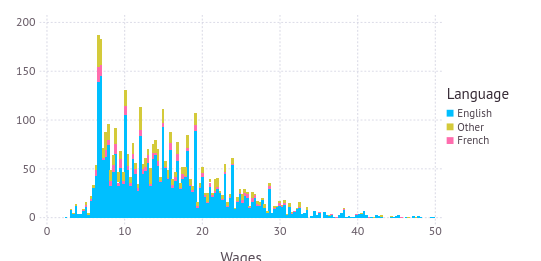
\includegraphics[width=0.6\textwidth]{gadfly0}
  \end{figure}
\end{frame}

\begin{frame}[fragile]
	\frametitle{Gadfly}
  \begin{tiny}
  \begin{minted}{julia}
using Gadfly
using RDatasets

iris = dataset("datasets", "iris")
p = plot(iris, x=:SepalLength, y=:SepalWidth, Geom.point);
img = SVG("iris_plot.svg", 6inch, 4inch)
draw(img, p)
  \end{minted}
  \end{tiny}
  \begin{figure}[ht]
    \centering
    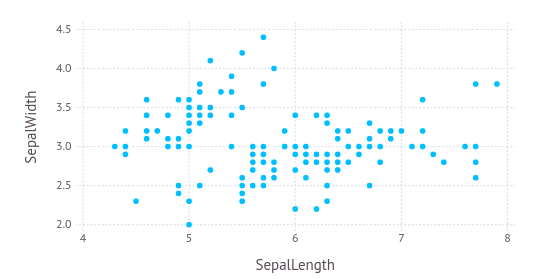
\includegraphics[width=0.6\textwidth]{gadfly1}
  \end{figure}
\end{frame}

\begin{frame}[fragile]
	\frametitle{Gadfly}
  \begin{tiny}
  \begin{minted}{julia}
fig1a = plot(iris, x="SepalLength", y="SepalWidth", Geom.point)
fig1b = plot(iris, x="SepalWidth", Geom.bar)
fig1 = hstack(fig1a, fig1b)
  \end{minted}
  \end{tiny}
  \begin{figure}[ht]
    \centering
    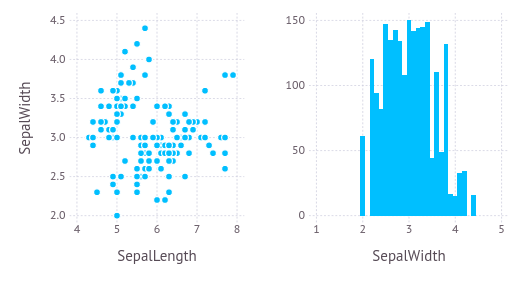
\includegraphics[width=0.6\textwidth]{gadfly2}
  \end{figure}
\end{frame}

\begin{frame}[fragile]
	\frametitle{Gadfly}
  \begin{tiny}
  \begin{minted}{julia}
using DataFrames

xs = 0:0.1:20

df_cos = DataFrame(x=xs,y=cos(xs),ymin=cos(xs) .- 0.5,ymax=cos(xs) .+ 0.5,f="cos")

df_sin = DataFrame(x=xs,y=sin(xs),ymin=sin(xs) .- 0.5,ymax=sin(xs) .+ 0.5,f="sin")

df = vcat(df_cos, df_sin)
p = plot(df, x=:x, y=:y, ymin=:ymin, ymax=:ymax, color=:f, Geom.line, Geom.ribbon)
  \end{minted}
  \end{tiny}
  \begin{figure}[ht]
    \centering
    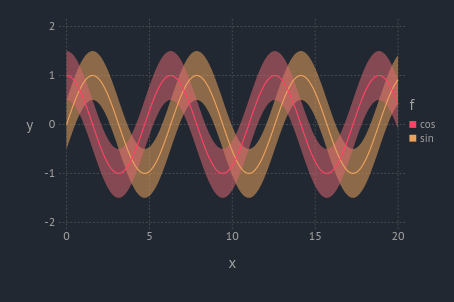
\includegraphics[width=0.5\textwidth]{gadfly3}
  \end{figure}
\end{frame}

\begin{frame}[fragile]
	\frametitle{Mocha}
  \begin{tiny}
  \begin{minted}{julia}
using Mocha

data  = HDF5DataLayer(name="train-data",source="train-data-list.txt",batch_size=64)
conv  = ConvolutionLayer(name="conv1",n_filter=20,kernel=(5,5),bottoms=[:data],tops=[:conv])
pool  = PoolingLayer(name="pool1",kernel=(2,2),stride=(2,2),bottoms=[:conv],tops=[:pool])
conv2 = ConvolutionLayer(name="conv2",n_filter=50,kernel=(5,5),bottoms=[:pool],tops=[:conv2])
pool2 = PoolingLayer(name="pool2",kernel=(2,2),stride=(2,2),bottoms=[:conv2],tops=[:pool2])
fc1   = InnerProductLayer(name="ip1",output_dim=500,neuron=Neurons.ReLU(),bottoms=[:pool2],
                          tops=[:ip1])
fc2   = InnerProductLayer(name="ip2",output_dim=10,bottoms=[:ip1],tops=[:ip2])
loss  = SoftmaxLossLayer(name="loss",bottoms=[:ip2,:label])

backend = DefaultBackend()
init(backend)

common_layers = [conv, pool, conv2, pool2, fc1, fc2]
net = Net("MNIST-train", backend, [data, common_layers..., loss])

exp_dir = "snapshots"
solver_method = SGD()
params = make_solver_parameters(solver_method, max_iter=10000, regu_coef=0.0005,
    mom_policy=MomPolicy.Fixed(0.9),
    lr_policy=LRPolicy.Inv(0.01, 0.0001, 0.75),
    load_from=exp_dir)
solver = Solver(solver_method, params)
  \end{minted}
  \end{tiny}
\end{frame}

\begin{frame}[fragile]
	\frametitle{Mocha}
  \begin{tiny}
  \begin{minted}{julia}
setup_coffee_lounge(solver, save_into="$exp_dir/statistics.jld", every_n_iter=1000)

# report training progress every 100 iterations
add_coffee_break(solver, TrainingSummary(), every_n_iter=100)

# save snapshots every 5000 iterations
add_coffee_break(solver, Snapshot(exp_dir), every_n_iter=5000)

# show performance on test data every 1000 iterations
data_test = HDF5DataLayer(name="test-data",source="test-data-list.txt",batch_size=100)
accuracy = AccuracyLayer(name="test-accuracy",bottoms=[:ip2, :label])
test_net = Net("MNIST-test", backend, [data_test, common_layers..., accuracy])
add_coffee_break(solver, ValidationPerformance(test_net), every_n_iter=1000)

solve(solver, net)

destroy(net)
destroy(test_net)
shutdown(backend)
  \end{minted}
  \end{tiny}
\end{frame}

\section{Conclusion}
\frame
{
	\frametitle{Where to go from here}
  \begin{itemize}
    \item Read the official Julia manual
    \item Accept the speedbumps
    \item Join the community
    \item Questions?
    \item https://github.com/d9w/julia-present
  \end{itemize}
}


\end{document}
